%\VignetteIndexEntry{Bioconductor LaTeX Style}
%\VignettePackage{BiocStyle}
%\VignetteEngine{knitr::knitr}

\documentclass{article}\usepackage[]{graphicx}\usepackage[usenames,dvipsnames]{color}
%% maxwidth is the original width if it is less than linewidth
%% otherwise use linewidth (to make sure the graphics do not exceed the margin)
\makeatletter
\def\maxwidth{ %
  \ifdim\Gin@nat@width>\linewidth
    \linewidth
  \else
    \Gin@nat@width
  \fi
}
\makeatother

\definecolor{fgcolor}{rgb}{0.345, 0.345, 0.345}
\newcommand{\hlnum}[1]{\textcolor[rgb]{0.686,0.059,0.569}{#1}}%
\newcommand{\hlstr}[1]{\textcolor[rgb]{0.192,0.494,0.8}{#1}}%
\newcommand{\hlcom}[1]{\textcolor[rgb]{0.678,0.584,0.686}{\textit{#1}}}%
\newcommand{\hlopt}[1]{\textcolor[rgb]{0,0,0}{#1}}%
\newcommand{\hlstd}[1]{\textcolor[rgb]{0.345,0.345,0.345}{#1}}%
\newcommand{\hlkwa}[1]{\textcolor[rgb]{0.161,0.373,0.58}{\textbf{#1}}}%
\newcommand{\hlkwb}[1]{\textcolor[rgb]{0.69,0.353,0.396}{#1}}%
\newcommand{\hlkwc}[1]{\textcolor[rgb]{0.333,0.667,0.333}{#1}}%
\newcommand{\hlkwd}[1]{\textcolor[rgb]{0.737,0.353,0.396}{\textbf{#1}}}%
\let\hlipl\hlkwb

\usepackage{framed}
\makeatletter
\newenvironment{kframe}{%
 \def\at@end@of@kframe{}%
 \ifinner\ifhmode%
  \def\at@end@of@kframe{\end{minipage}}%
  \begin{minipage}{\columnwidth}%
 \fi\fi%
 \def\FrameCommand##1{\hskip\@totalleftmargin \hskip-\fboxsep
 \colorbox{shadecolor}{##1}\hskip-\fboxsep
     % There is no \\@totalrightmargin, so:
     \hskip-\linewidth \hskip-\@totalleftmargin \hskip\columnwidth}%
 \MakeFramed {\advance\hsize-\width
   \@totalleftmargin\z@ \linewidth\hsize
   \@setminipage}}%
 {\par\unskip\endMakeFramed%
 \at@end@of@kframe}
\makeatother

\definecolor{shadecolor}{rgb}{.97, .97, .97}
\definecolor{messagecolor}{rgb}{0, 0, 0}
\definecolor{warningcolor}{rgb}{1, 0, 1}
\definecolor{errorcolor}{rgb}{1, 0, 0}
\newenvironment{knitrout}{}{} % an empty environment to be redefined in TeX

\usepackage{alltt}

\RequirePackage{/usr/local/lib/R/site-library/BiocStyle/resources/tex/Bioconductor}

\AtBeginDocument{\bibliographystyle{/usr/local/lib/R/site-library/BiocStyle/resources/tex/unsrturl}}


\renewcommand{\baselinestretch}{1.25}

\newcommand{\exitem}[3]{%
  \item \texttt{\textbackslash#1\{#2\}} #3 \csname#1\endcsname{#2}.%
}

\bioctitle[powsimR]{powsimR: Power Analysis and Sample Size Estimation for Bulk and Single Cell RNA-Seq Experiments}
\author{Beate Vieth \footnote{vieth@bio.lmu.de}}
\IfFileExists{upquote.sty}{\usepackage{upquote}}{}
\begin{document}

\maketitle

%\packageVersion{BiocStyle::pkg_ver("powsimR")}

Report issues on \url{https://github.com/bvieth/powsimR/issues}

\newpage

\tableofcontents



\newpage

%---------------------------------------------------------
\section{Installation guide}
%---------------------------------------------------------

PowsimR has a number of dependencies that need to be installed before hand (see also the README file on github). I recommend to increase the maximum number of DLLs that can be loaded to at least 500. The environmental variable R\_MAX\_NUM\_DLLS can be set in R\_HOME/etc/Renviron prior to starting R (for further details see \Rfunction{Startup}).

\begin{knitrout}
\definecolor{shadecolor}{rgb}{0.969, 0.969, 0.969}\color{fgcolor}\begin{kframe}
\begin{alltt}
\hlstd{ipak} \hlkwb{<-} \hlkwa{function}\hlstd{(}\hlkwc{pkg}\hlstd{,} \hlkwc{repository} \hlstd{=} \hlkwd{c}\hlstd{(}\hlstr{"CRAN"}\hlstd{,} \hlstr{"Bioconductor"}\hlstd{,}
    \hlstr{"github"}\hlstd{)) \{}
    \hlstd{new.pkg} \hlkwb{<-} \hlstd{pkg[}\hlopt{!}\hlstd{(pkg} \hlopt \hlkwd{installed.packages}\hlstd{()[,} \hlstr{"Package"}\hlstd{])]}
    \hlkwa{if} \hlstd{(}\hlkwd{length}\hlstd{(new.pkg)) \{}
        \hlkwa{if} \hlstd{(repository} \hlopt{==} \hlstr{"CRAN"}\hlstd{) \{}
            \hlkwd{install.packages}\hlstd{(new.pkg,} \hlkwc{dependencies} \hlstd{=} \hlnum{TRUE}\hlstd{)}
        \hlstd{\}}
        \hlkwa{if} \hlstd{(repository} \hlopt{==} \hlstr{"Bioconductor"}\hlstd{) \{}
            \hlkwd{source}\hlstd{(}\hlstr{"https://bioconductor.org/biocLite.R"}\hlstd{)}
            \hlkwd{biocLite}\hlstd{(new.pkg,} \hlkwc{dependencies} \hlstd{=} \hlnum{TRUE}\hlstd{,} \hlkwc{ask} \hlstd{=} \hlnum{FALSE}\hlstd{)}
        \hlstd{\}}
        \hlkwa{if} \hlstd{(repository} \hlopt{==} \hlstr{"github"}\hlstd{) \{}
            \hlstd{devtools}\hlopt{::}\hlkwd{install_github}\hlstd{(pkg,} \hlkwc{build_vignettes} \hlstd{=} \hlnum{FALSE}\hlstd{)}
        \hlstd{\}}
    \hlstd{\}}
\hlstd{\}}

\hlcom{# CRAN PACKAGES}
\hlstd{cranpackages} \hlkwb{<-} \hlkwd{c}\hlstd{(}\hlstr{"gamlss.dist"}\hlstd{,} \hlstr{"methods"}\hlstd{,} \hlstr{"stats"}\hlstd{,} \hlstr{"moments"}\hlstd{,}
    \hlstr{"doParallel"}\hlstd{,} \hlstr{"parallel"}\hlstd{,} \hlstr{"reshape2"}\hlstd{,} \hlstr{"dplyr"}\hlstd{,} \hlstr{"tidyr"}\hlstd{,} \hlstr{"data.table"}\hlstd{,}
    \hlstr{"ggplot2"}\hlstd{,} \hlstr{"ggthemes"}\hlstd{,} \hlstr{"ggExtra"}\hlstd{,} \hlstr{"cowplot"}\hlstd{,} \hlstr{"scales"}\hlstd{,} \hlstr{"fitdistrplus"}\hlstd{,}
    \hlstr{"MASS"}\hlstd{,} \hlstr{"pscl"}\hlstd{,} \hlstr{"nonnest2"}\hlstd{,} \hlstr{"cobs"}\hlstd{,} \hlstr{"msir"}\hlstd{,} \hlstr{"drc"}\hlstd{,} \hlstr{"devtools"}\hlstd{,}
    \hlstr{"XML"}\hlstd{,} \hlstr{"splines"}\hlstd{,} \hlstr{"gtools"}\hlstd{,} \hlstr{"NBPSeq"}\hlstd{)}
\hlkwd{ipak}\hlstd{(cranpackages,} \hlkwc{repository} \hlstd{=} \hlstr{"CRAN"}\hlstd{)}

\hlcom{# BIOCONDUCTOR}
\hlstd{biocpackages} \hlkwb{<-} \hlkwd{c}\hlstd{(}\hlstr{"S4Vectors"}\hlstd{,} \hlstr{"AnnotationDbi"}\hlstd{,} \hlstr{"Biobase"}\hlstd{,} \hlstr{"BiocParallel"}\hlstd{,}
    \hlstr{"BiocStyle"}\hlstd{,} \hlstr{"scater"}\hlstd{,} \hlstr{"scran"}\hlstd{,} \hlstr{"edgeR"}\hlstd{,} \hlstr{"limma"}\hlstd{,} \hlstr{"DESeq2"}\hlstd{,}
    \hlstr{"baySeq"}\hlstd{,} \hlstr{"NOISeq"}\hlstd{,} \hlstr{"EBSeq"}\hlstd{,} \hlstr{"DSS"}\hlstd{,} \hlstr{"MAST"}\hlstd{,} \hlstr{"ROTS"}\hlstd{,} \hlstr{"IHW"}\hlstd{,}
    \hlstr{"qvalue"}\hlstd{,} \hlstr{"scDD"}\hlstd{,} \hlstr{"monocle"}\hlstd{,} \hlstr{"RUVSeq"}\hlstd{)}
\hlkwd{ipak}\hlstd{(biocpackages,} \hlkwc{repository} \hlstd{=} \hlstr{"Bioconductor"}\hlstd{)}

\hlcom{# GITHUB}
\hlstd{githubpackages} \hlkwb{<-} \hlkwd{c}\hlstd{(}\hlstr{"gu-mi/NBGOF"}\hlstd{,} \hlstr{"hms-dbmi/scde"}\hlstd{,} \hlstr{"nghiavtr/BPSC"}\hlstd{,}
    \hlstr{"rhondabacher/SCnorm"}\hlstd{,} \hlstr{"catavallejos/BASiCS"}\hlstd{)}
\hlkwd{ipak}\hlstd{(githubpackages,} \hlkwc{repository} \hlstd{=} \hlstr{"github"}\hlstd{)}
\end{alltt}
\end{kframe}
\end{knitrout}

After installing the dependencies, \Rpackage{powsimR} can be installed by using devtools as well.

\begin{knitrout}
\definecolor{shadecolor}{rgb}{0.969, 0.969, 0.969}\color{fgcolor}\begin{kframe}
\begin{alltt}
\hlstd{devtools}\hlopt{::}\hlkwd{install_github}\hlstd{(}\hlstr{"bvieth/powsimR"}\hlstd{,} \hlkwc{build_vignettes} \hlstd{=} \hlnum{TRUE}\hlstd{)}
\end{alltt}
\end{kframe}
\end{knitrout}


%---------------------------------------------------------
\section{Introduction}
%---------------------------------------------------------

In this vignette, we illustrate the features of \Rpackage{powsimR} by assessing the power to detect differential expression between two groups of embryonic stem cells cultured in standard 2i medium (\href{http://www.ebi.ac.uk/arrayexpress/experiments/E-MTAB-2600/}{E-MTAB-2600}) \cite{Kolodziejczyk2015-vn}.

%---------------------------------------------------------
\section{\Rpackage{powsimR} workflow}
%---------------------------------------------------------

The basic workflow of \Rpackage{powsimR} is illustrated in figure \ref{fig:powsim_scheme}: A) The mean-dispersion relationship is estimated from RNA-seq data, which can be either single cell or bulk data. The users can provide their own count tables or one of our five example data sets. B) These distribution parameters are then used to set-up the simulations. For better comparability, the parameters for the simulation of differential expression are set separately. C) Finally, the TPR and FDR are calculated. Both can be either returned as marginal estimates per sample configuration (shown), or stratified according to the estimates of mean expression, dispersion or dropout rate.

\begin{figure}[h]
\centering
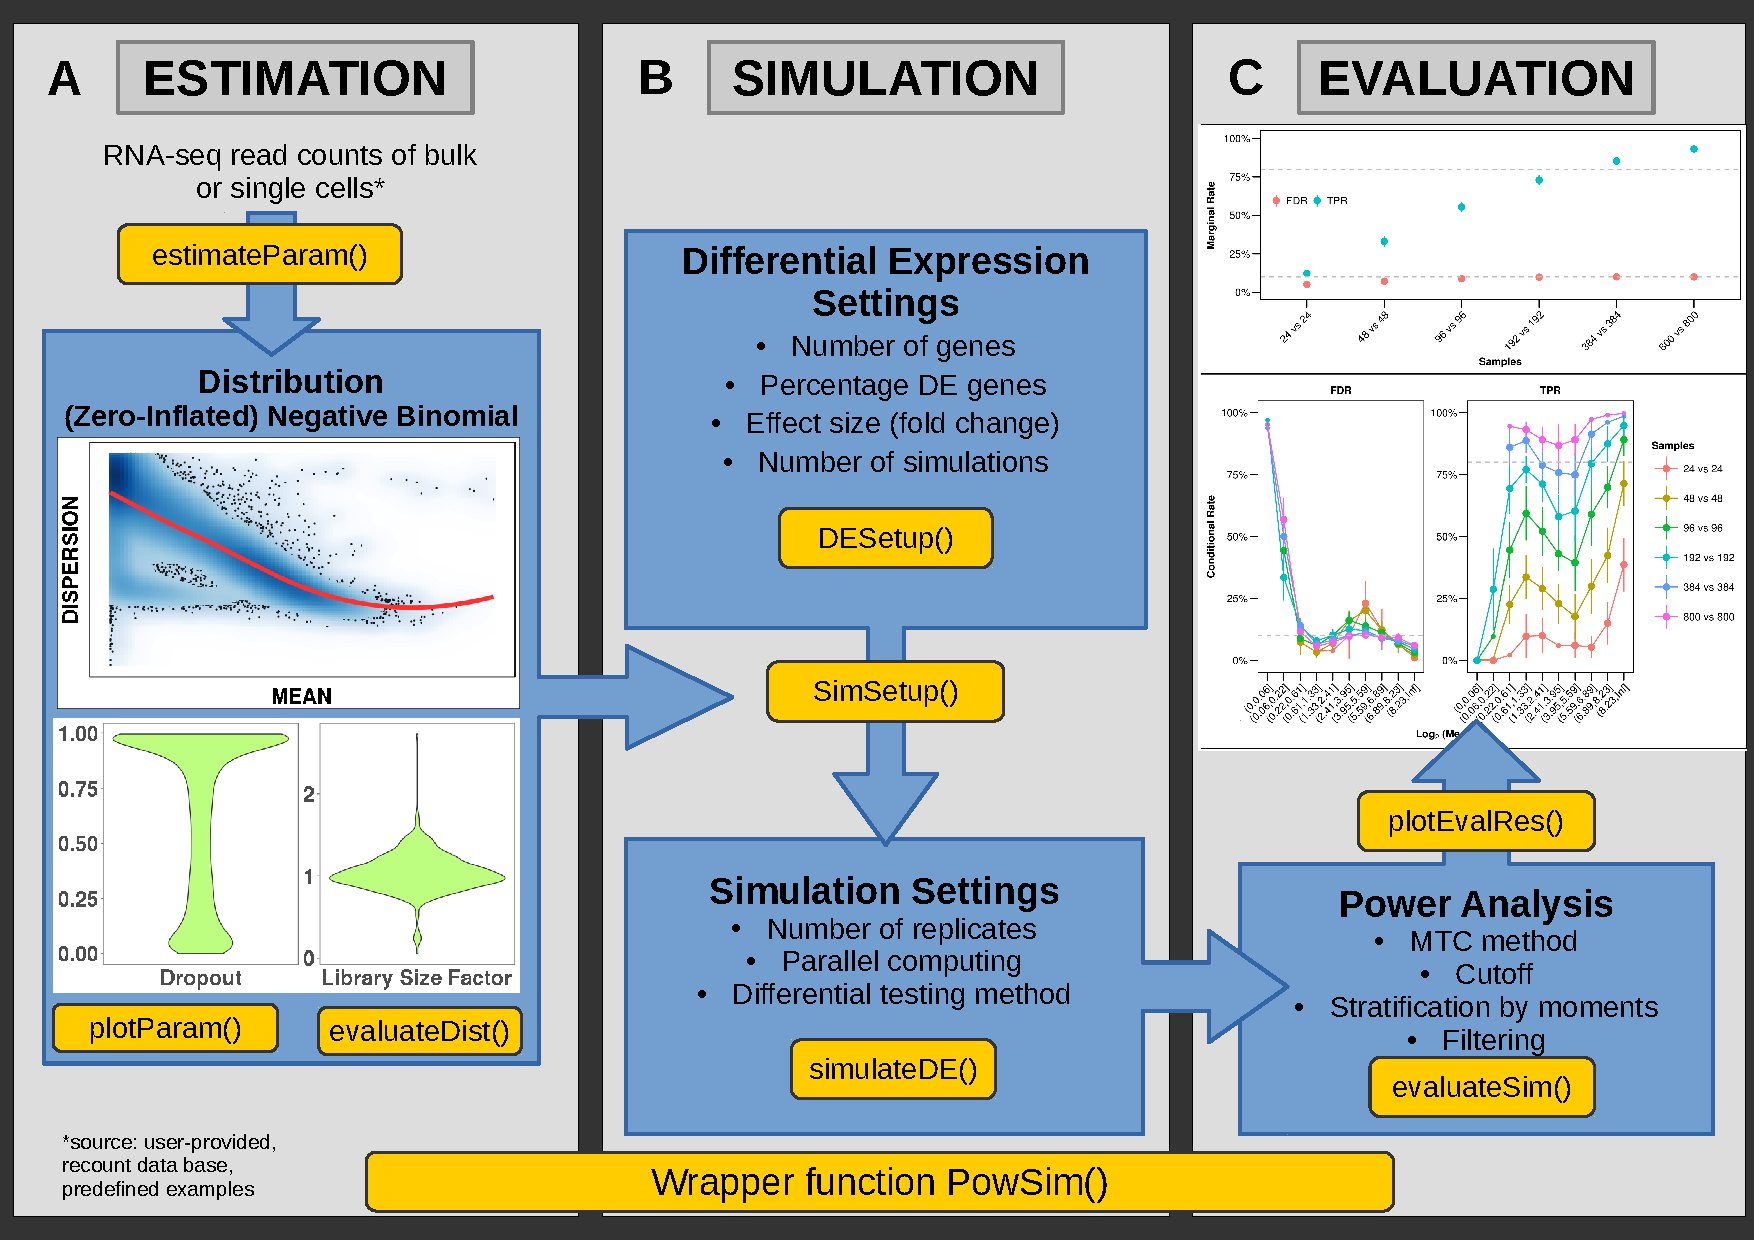
\includegraphics[width=0.95\linewidth]{powsim_schematic.pdf}
\caption{\textbf{PowsimR schematic overview.} (A) Estimation: (B) Simulation: (C) Evaluation. Functions given in orange.}
\label{fig:powsim_scheme}
\end{figure}

\section{Parameter Estimation}

The parameters of the negative binomial distribution, i.e. mean and dispersion are estimated by the function \Rfunction{estimateParam}. In addition, the dropout probability, i.e. the fraction of zero counts per gene, is calculated.
The user can choose between two estimation frameworks:
\begin{description}
\item[NB] Negative binomial distribution.
\item[ZINB] Zero-inflated negative binomial distribution.
\item[MatchMoments] Matching moments estimation of mean and dispersion based on normalized counts.
\end{description}

In both cases matching moments estimation of mean and dispersion are based on normalized counts.

The user can choose between multiple normalisation methods (see details section of \Rfunction{estimateParam}).

The estimates, sequencing depth and normalisation factors are plotted with \Rfunction{plotParam}.

With the following command, we estimate and plot the parameters for the embryonic stem cells cultured in standard 2i+lif medium (Kolodziejczyk) (figure \ref{fig:NBparams}). As expected for single cell RNA-seq, the variability (i.e. dispersion) and dropout rates are high. Furthermore, the dispersion strongly depends on the mean and does not level off with higher mean values.

\begin{knitrout}
\definecolor{shadecolor}{rgb}{0.969, 0.969, 0.969}\color{fgcolor}\begin{kframe}
\begin{alltt}
\hlcom{# download count table}
\hlstd{githubURL} \hlkwb{<-} \hlstr{"https://github.com/bvieth/powsimRData/raw/master/data-raw/kolodziejczk_cnts.rda"}
\hlkwd{download.file}\hlstd{(}\hlkwc{url} \hlstd{= githubURL,} \hlkwc{destfile} \hlstd{=} \hlstr{"kolodziejczk_cnts.rda"}\hlstd{,}
    \hlkwc{method} \hlstd{=} \hlstr{"wget"}\hlstd{)}
\hlkwd{load}\hlstd{(}\hlstr{"kolodziejczk_cnts.rda"}\hlstd{)}
\hlstd{kolodziejczk_cnts} \hlkwb{<-} \hlstd{kolodziejczk_cnts[,} \hlkwd{grep}\hlstd{(}\hlstr{"standard"}\hlstd{,} \hlkwd{colnames}\hlstd{(kolodziejczk_cnts))]}

\hlstd{TwoiLIF.params} \hlkwb{<-} \hlkwd{estimateParam}\hlstd{(}\hlkwc{countData} \hlstd{= kolodziejczk_cnts,}
    \hlkwc{spikeData} \hlstd{=} \hlkwa{NULL}\hlstd{,} \hlkwc{spikeInfo} \hlstd{=} \hlkwa{NULL}\hlstd{,} \hlkwc{Lengths} \hlstd{=} \hlkwa{NULL}\hlstd{,} \hlkwc{MeanFragLengths} \hlstd{=} \hlkwa{NULL}\hlstd{,}
    \hlkwc{Distribution} \hlstd{=} \hlstr{"NB"}\hlstd{,} \hlkwc{RNAseq} \hlstd{=} \hlstr{"singlecell"}\hlstd{,} \hlkwc{normalisation} \hlstd{=} \hlstr{"scran"}\hlstd{,}
    \hlkwc{NCores} \hlstd{=} \hlkwa{NULL}\hlstd{,} \hlkwc{sigma} \hlstd{=} \hlnum{1.96}\hlstd{)}
\hlkwd{plotParam}\hlstd{(TwoiLIF.params)}
\end{alltt}
\end{kframe}
\end{knitrout}

We have implemented a read count simulation framework assuming either a negative binomial distribution or a zero-inflated negative binomial distribution.
To predict the dispersion given a random draw of mean expression value observed, we apply a locally weighted polynomial regression fit. To capture the variability of dispersion estimates observed, a local variability prediction band is applied.
For bulk RNA-seq experiments, dropouts are less probable but can still occur. To include this phenomenon we sample from the observed dropout rates for genes that have a mean expression value below 5\% dropout probability determined by a decrease constrained B-splines regresssion of dropout rate against mean expression (\Rfunction{cobs} in \CRANpkg{cobs}).
The resulting read count matrix has similar distributional characteristics as the original Kolodziejczyk data set (figure \ref{fig:simeval}).
For the zero-inflated negative binomial distribution, the mean-dispersion relation is similarly estimated, but based on positive read counts. Furthermore, the dropouts are also predicted based on a locally weighted polynomial regression fit between mean and dropouts. Of note, this fit is done separately for amplified and non-amplified transcripts separately and similar proportions of genes as observed are also generated in the simulations \cite{Ziegenhain2017-sf}.
We have found that the negative binomial distribution is particularly suited for UMI-methods (e.g. SCRB-Seq, Drop-Seq, 10XGenomics) \cite{Vieth2017-su}.


\begin{figure}[h]
\centering
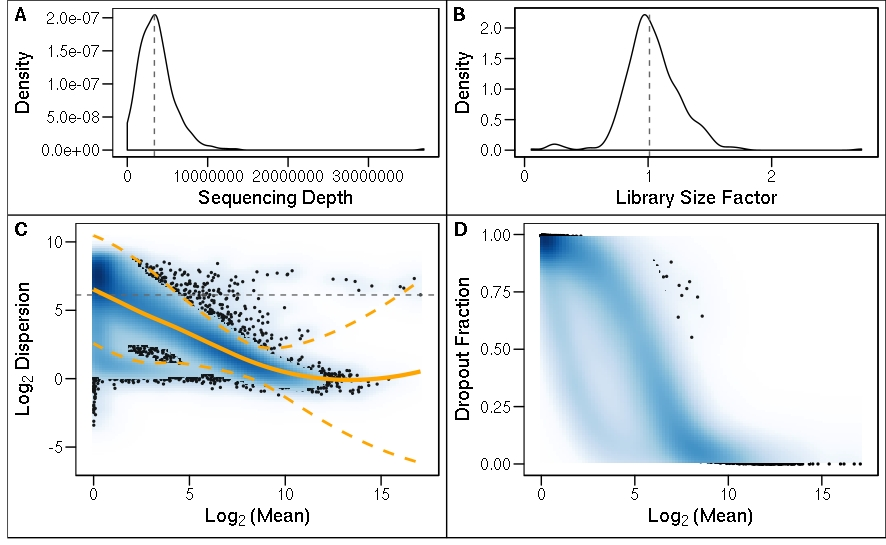
\includegraphics[width=0.75\linewidth]{NBparams.jpeg}
\caption{\textbf{Estimated parameters for Kolodziejczyk data set.} A) Sequencing depth per sample with median sequencing depth (grey dashed line). B) Library size normalisation factor per sample with median size factor (grey dashed line). C) Marginal Distribution of mean, dispersion and dropout. D) Local polynomial regression fit between mean and dispersion estimates with variability band per gene (yellow). Common dispersion estimate (grey dashed line). E) Fraction of dropouts versus estimated mean expression per gene.}
\label{fig:NBparams}
\end{figure}

\begin{figure}[h]
\centering
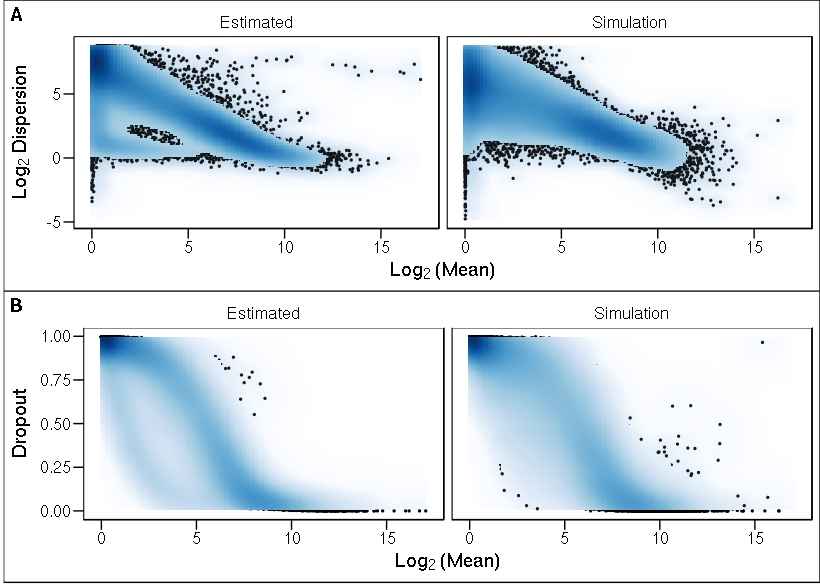
\includegraphics[width=0.7\linewidth]{simeval.jpeg}
\caption{\textbf{Comparison of estimated and simulated read counts} (A) Dispersion versus Mean. (B) Dropout versus Mean.}
\label{fig:simeval}
\end{figure}

%---------------------------------------------------------
\section{Simulations}
%---------------------------------------------------------
For simulating differential expression between two groups, the number of genes, number of simulations, percentage of differential expression and effect size are set up with the function \Rfunction{DESetup}. The effect size is here defined as the log2 fold change which can be a constant, sampled from a vector or function. The uniform, normal and gamma distributions are possible options and illustrated in figure \ref{fig:lfcs}. Depending on the settings, these distribution can be broader or narrower. If using this option, we recommend to choose a distribution that closely resembles previously observed or expected fold changes.

The distribution estimates and these settings are then combined to one object with \Rfunction{SimSetup}. This allows the user to assess power of multiple groupwise comparisons and different differential testing methods.
The following command sets up simulations with 10,000 genes, 20\% genes being DE, log fold change sample from a narrow gamma distribution and parameter estimates based on Kolodziejczyk data:

\begin{knitrout}
\definecolor{shadecolor}{rgb}{0.969, 0.969, 0.969}\color{fgcolor}\begin{kframe}
\begin{alltt}
\hlstd{lfc.gamma} \hlkwb{=} \hlkwa{function}\hlstd{(}\hlkwc{x}\hlstd{)} \hlkwd{sample}\hlstd{(}\hlkwd{c}\hlstd{(}\hlopt{-}\hlnum{1}\hlstd{,} \hlnum{1}\hlstd{),} \hlkwc{size} \hlstd{= x,} \hlkwc{replace} \hlstd{= T)} \hlopt{*}
    \hlkwd{rgamma}\hlstd{(x,} \hlnum{3}\hlstd{,} \hlnum{3}\hlstd{)}
\hlstd{de.opts} \hlkwb{=} \hlkwd{DESetup}\hlstd{(}\hlkwc{ngenes} \hlstd{=} \hlnum{10000}\hlstd{,} \hlkwc{nsims} \hlstd{=} \hlnum{25}\hlstd{,} \hlkwc{p.DE} \hlstd{=} \hlnum{0.2}\hlstd{,} \hlkwc{LFC} \hlstd{= lfc.gamma)}
\hlstd{sim.opts} \hlkwb{=} \hlkwd{SimSetup}\hlstd{(}\hlkwc{desetup} \hlstd{= de.opts,} \hlkwc{params} \hlstd{= TwoiLIF.params,}
    \hlkwc{size.factors} \hlstd{=} \hlstr{"given"}\hlstd{,} \hlkwc{normalisation} \hlstd{=} \hlstr{"scran"}\hlstd{)}
\end{alltt}
\end{kframe}
\end{knitrout}

With the setup defined, the differential expression simulation is run with \Rfunction{simulateDE}. For this, the user needs to set the following options:

\begin{description}
  \item[Replicates] The number of sample replicates per group (n1 and n2). These can be unbalanced.
  \item[DEmethod] The differential testing method. The user can choose between 12 methods in total.  8 developed for bulk, 4 developed for single cells (see the detail section of \Rfunction{simulateDE}).
  \item[ncores] A number of DE methods are able to run in parallel to speed up differential testing.
\end{description}

\begin{knitrout}
\definecolor{shadecolor}{rgb}{0.969, 0.969, 0.969}\color{fgcolor}\begin{kframe}
\begin{alltt}
\hlstd{simDE} \hlkwb{=} \hlkwd{simulateDE}\hlstd{(}\hlkwc{n1} \hlstd{=} \hlkwd{c}\hlstd{(}\hlnum{24}\hlstd{,} \hlnum{48}\hlstd{,} \hlnum{96}\hlstd{,} \hlnum{192}\hlstd{,} \hlnum{384}\hlstd{,} \hlnum{800}\hlstd{),} \hlkwc{n2} \hlstd{=} \hlkwd{c}\hlstd{(}\hlnum{24}\hlstd{,}
    \hlnum{48}\hlstd{,} \hlnum{96}\hlstd{,} \hlnum{192}\hlstd{,} \hlnum{384}\hlstd{,} \hlnum{800}\hlstd{),} \hlkwc{sim.settings} \hlstd{= sim.opts,} \hlkwc{ncores} \hlstd{=} \hlnum{10}\hlstd{,}
    \hlkwc{DEmethod} \hlstd{=} \hlstr{"MAST"}\hlstd{,} \hlkwc{verbose} \hlstd{= T)}
\end{alltt}
\end{kframe}
\end{knitrout}

\begin{figure}[h]
\centering
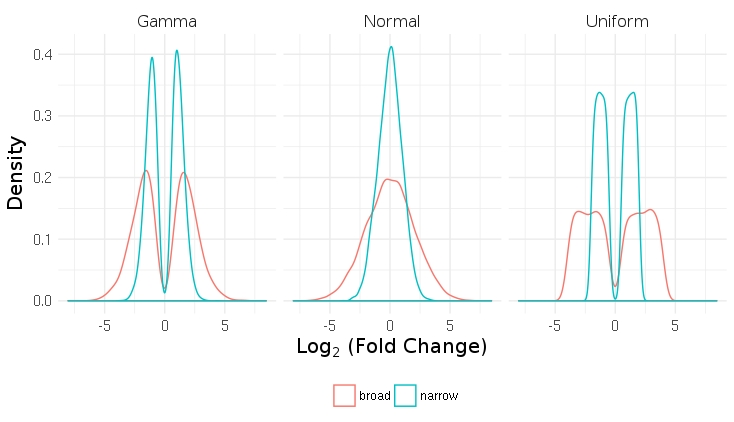
\includegraphics[width=0.6\linewidth]{lfcdist.jpeg}
\caption{Log2 fold change examples for gamma, uniform and normal distribution}
\label{fig:lfcs}
\end{figure}

\section{Evaluation}

The results of differential expression simulation are evaluated with \Rfunction{evaluateSim}. We have separated the evaluation from DE detection to allow the user to evaluate power in a comprehensive way as advocated by \cite{Wu2015-uj}.
In this function, the proporations and error rates are estimated. The rates can be stratified by mean, dispersion or dropout. Furthermore, the user can choose between different multiple testing correction methods (see \Rfunction{p.adjust.methods}, \Rfunction{ihw} in \Biocpkg{IHW} and \Rfunction{qvalue} in \Biocpkg{qvalue}). Also, the genes can be filtered by mean, dispersion or dropout. To define biologically interesting genes, a cutoff for the log2 fold change with delta can be set.

With the following command we evaluate the marginal TPR and FDR conditional on the mean expression for the simulation based on Kolodziejczyk data.

\begin{knitrout}
\definecolor{shadecolor}{rgb}{0.969, 0.969, 0.969}\color{fgcolor}\begin{kframe}
\begin{alltt}
\hlstd{evalDE} \hlkwb{=} \hlkwd{evaluateSim}\hlstd{(}\hlkwc{simRes} \hlstd{= simDE,} \hlkwc{alpha.type} \hlstd{=} \hlstr{"adjusted"}\hlstd{,}
    \hlkwc{MTC} \hlstd{=} \hlstr{"BH"}\hlstd{,} \hlkwc{alpha.nominal} \hlstd{=} \hlnum{0.1}\hlstd{,} \hlkwc{stratify.by} \hlstd{=} \hlstr{"mean"}\hlstd{,} \hlkwc{filter.by} \hlstd{=} \hlstr{"none"}\hlstd{,}
    \hlkwc{strata.filtered} \hlstd{=} \hlnum{0}\hlstd{,} \hlkwc{target.by} \hlstd{=} \hlstr{"lfc"}\hlstd{,} \hlkwc{delta} \hlstd{=} \hlnum{0}\hlstd{)}
\end{alltt}
\end{kframe}
\end{knitrout}

The results of the evaluation can be plotted with \Rfunction{plotEvalRes}.
\begin{description}
  \item[rate] Marginal or Conditional Error Rates calculations. The conditional error rates are determined and calculated with \Rfunction{evaluateSim}. The number of genes per stratum are also summarised.
  \item[quick] If this is set to \R{TRUE} then only the TPR and FDR will be plotted.
\end{description}

With the following commands, the quick marginal and conditional power assessment for the Kolodziejczyk data is plotted.

\begin{knitrout}
\definecolor{shadecolor}{rgb}{0.969, 0.969, 0.969}\color{fgcolor}\begin{kframe}
\begin{alltt}
\hlkwd{plotEvalRes}\hlstd{(}\hlkwc{evalRes} \hlstd{= evalDE,} \hlkwc{rate} \hlstd{=} \hlstr{"marginal"}\hlstd{,} \hlkwc{quick} \hlstd{=} \hlnum{TRUE}\hlstd{,}
    \hlkwc{annot} \hlstd{=} \hlnum{TRUE}\hlstd{)}

\hlkwd{plotEvalRes}\hlstd{(}\hlkwc{evalRes} \hlstd{= evalDE,} \hlkwc{rate} \hlstd{=} \hlstr{"stratified"}\hlstd{,} \hlkwc{quick} \hlstd{=} \hlnum{TRUE}\hlstd{,}
    \hlkwc{annot} \hlstd{=} \hlnum{TRUE}\hlstd{)}
\end{alltt}
\end{kframe}
\end{knitrout}

%---------------------------------------------------------
\section{Additional Functionalities}
%---------------------------------------------------------

\subsection{Evaluate Simulation Framework}

It is important to validate the appropiateness of the chosen simulation framework. The function \Rfunction{evaluateDist} compares the theoretical fit of the Poisson, negative binomial, zero-inflated Poisson and zero-inflated negative binomial and beta-Poisson distribution to the empirical RNA-seq read counts (\cite{Colin_Cameron2013-vb}, \cite{Kim2013-qo}, \cite{Delmans2016-ef}).
The evaluation is then plotted with the function \Rfunction{plotEvalDist} which summarizes the best fitting distribution per gene based on goodness-of-fit statistics (Chi-square test), Akaike Information Criterium, comparing observed dropouts with zero count prediction of the models and comparing the model fitness with Likelihood Ratio Test and Vuong Test.
% As noted by other developers, goodness-of-fit tests are not an objective tool and heavily depend on sample sizes (\cite{Delignette-Muller2015-ie}). A graphical evaluation of the fitted distribution is considered the most appropiate way but for high-throughput sequencing an unrealistic recommendation.
Bulk RNA-seq experiments are usually conducted with a small number of samples. We therefore recommend to rely on the goodness-of-fit validation by \cite{Mi2015-ri}. To use this approach in \Rfunction{evaluateDist}, the user should allow for permutation simulations by setting the value of nsims to at least 100. If available, the computation can be run on multiple cores by setting the number of cores (ncores).

With the following command, we estimate and plot the parameters for the embryonic stem cells cultured in standard 2i lif medium (Kolodziejczyk).

\begin{knitrout}
\definecolor{shadecolor}{rgb}{0.969, 0.969, 0.969}\color{fgcolor}\begin{kframe}
\begin{alltt}
\hlstd{TwoiLIF.distfit} \hlkwb{=} \hlkwd{evaluateDist}\hlstd{(}\hlkwc{cnts} \hlstd{= kolodziejczk_cnts,} \hlkwc{RNAseq} \hlstd{=} \hlstr{"singlecell"}\hlstd{,}
    \hlkwc{ncores} \hlstd{=} \hlnum{1}\hlstd{,} \hlkwc{nsims} \hlstd{=} \hlnum{1}\hlstd{,} \hlkwc{frac.genes} \hlstd{=} \hlnum{1}\hlstd{,} \hlkwc{min.meancount} \hlstd{=} \hlnum{1}\hlstd{,}
    \hlkwc{min.libsize} \hlstd{=} \hlnum{1000}\hlstd{)}

\hlkwd{plotEvalDist}\hlstd{(}\hlkwc{evalDist} \hlstd{= TwoiLIF.distfit,} \hlkwc{annot} \hlstd{= F)}
\end{alltt}
\end{kframe}
\end{knitrout}

\begin{figure}[h]
\centering
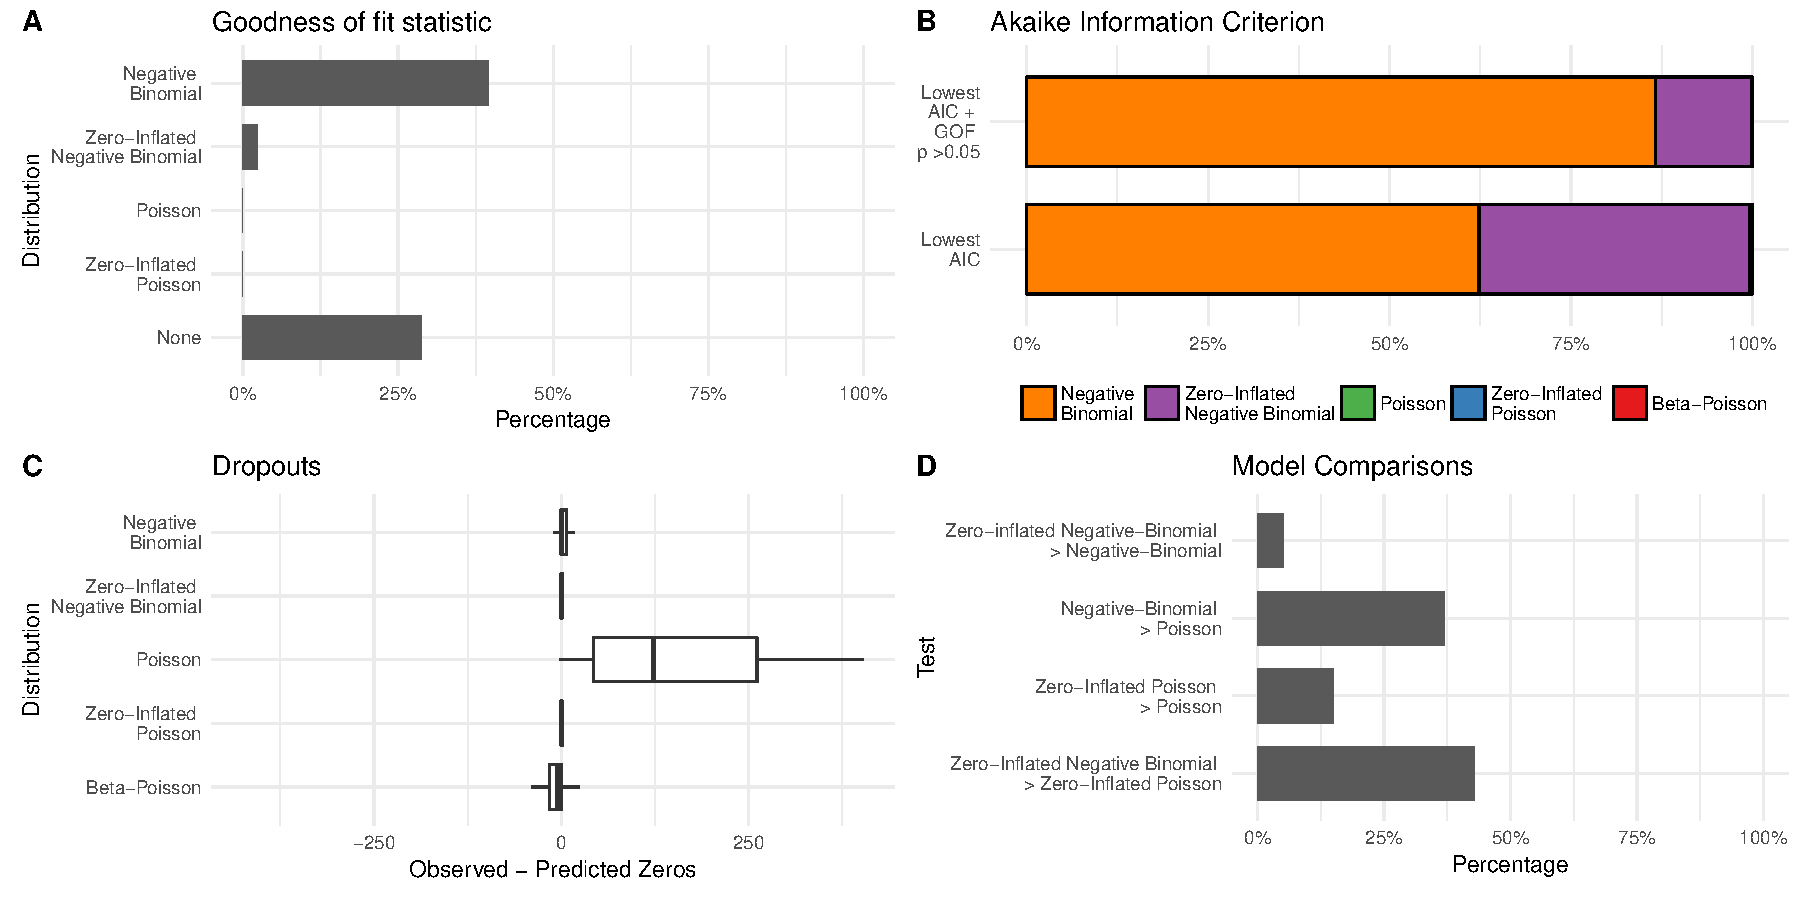
\includegraphics[width=0.75\linewidth]{evaldist.pdf}
\caption{A) Goodness of fit of the model per gene assessed with a Chi-square test based on residual deviance and degrees of freedom. B) The fraction of genes for which the respective distribution has the lowest AIC and additionally the distribution with the lowest AIC as well as not rejected by the goodness of fit statistic.  C) Observed versus predicted dropouts per distributional model and gene. D) Model assessment per gene based on Likelihood Ratio Test for nested models and Vung Test for non-nested models.}
\label{fig:evaldist}
\end{figure}

\subsection{Negative Binomial Parameters}

\subsubsection{in silico Parameter Definition}

We have also implemented the option to approximate the read count matrix simulation based on random distribution functions in \R{}. The user then has to define the mean, dispersion, dropout and library size in \Rfunction{insilicoNBParam}. In the absence of suitable pilot studies, a typical single cell RNA-seq experiment could be approximated with:
\begin{itemize}
  \item mean: \Rcode{function(x) rgamma(x, 4, 2)} where x is the number of genes
  \item dispersion: \Rcode{function(x) 2 + 100/x} where x is the mean
  \item library size: \Rcode{function(x) 2**rnorm(n=x, mean=0, sd=0.25)} where x is the number of samples
\end{itemize}

The same functionality can also be used for bulk RNA-seq.

\subsubsection{Count matrices of single cell RNA-seq experiments}

We have uploaded read count matrices of 5 single cell RNA-seq experiments on \href{https://github.com/bvieth/powsimRData}{github}.
The user can calculate the negative binomial parameters with \Rfunction{estimateParam}, view these estimates with \Rfunction{plotParam} and use it as an input for \Rfunction{SimSetup}.

\subsubsection{Access to raw read counts stored in online data base}

We have provided a number of exemplatory single cell RNA-seq data sets for parameter estimation. Nevertheless, you might not find a data set that matches your own experimental setup. In those cases, we recommend to check online repositories for a suitable data set. Below you can find an example script to get count tables from recount (\url{https://jhubiostatistics.shinyapps.io/recount/}) \cite{Collado-Torres2017-mo}. For a single cell RNA-seq data base, see conquer and its tutorial (\url{http://imlspenticton.uzh.ch:3838/conquer/}).
As before, the user can then calculate the negative binomial parameters with \Rfunction{estimateParam}, view these estimates with \Rfunction{plotParam} and use it as an input for \Rfunction{SimSetup}.

\begin{knitrout}
\definecolor{shadecolor}{rgb}{0.969, 0.969, 0.969}\color{fgcolor}\begin{kframe}
\begin{alltt}
\hlcom{# Install and load the R package}
\hlkwd{source}\hlstd{(}\hlstr{"http://bioconductor.org/biocLite.R"}\hlstd{)}
\hlkwd{biocLite}\hlstd{(}\hlstr{"recount"}\hlstd{)}
\hlkwd{library}\hlstd{(}\hlstr{"recount"}\hlstd{)}

\hlcom{# Download the data set}
\hlstd{url} \hlkwb{<-} \hlkwd{download_study}\hlstd{(}\hlstr{"SRP060416"}\hlstd{)}

\hlcom{# Load the data}
\hlkwd{load}\hlstd{(}\hlkwd{file.path}\hlstd{(}\hlstr{"SRP060416"}\hlstd{,} \hlstr{"rse_gene.Rdata"}\hlstd{))}

\hlcom{# count table}
\hlstd{cnts} \hlkwb{<-} \hlkwd{assay}\hlstd{(rse_gene)}
\hlcom{# sample annotation}
\hlstd{sample.info} \hlkwb{<-} \hlkwd{data.frame}\hlstd{(}\hlkwd{colData}\hlstd{(rse_gene)}\hlopt{@}\hlkwc{listData}\hlstd{,} \hlkwc{stringsAsFactors} \hlstd{= F)}
\hlcom{# gene annotation}
\hlstd{gene.info} \hlkwb{<-} \hlkwd{data.frame}\hlstd{(}\hlkwc{GeneID} \hlstd{=} \hlkwd{rowData}\hlstd{(rse_gene)}\hlopt{@}\hlkwc{listData}\hlopt{$}\hlstd{gene_id,}
    \hlkwc{GeneLength} \hlstd{=} \hlkwd{rowData}\hlstd{(rse_gene)}\hlopt{@}\hlkwc{listData}\hlopt{$}\hlstd{bp_length,} \hlkwc{stringsAsFactors} \hlstd{= F)}
\end{alltt}
\end{kframe}
\end{knitrout}


\subsection{Simulation settings}

By default, there is no difference in library sizes between the samples. If the user wishes for a more realistic, i.e. more variable distribution of read counts across samples, the library sizes can be sampled from observed, vector or function.

% %---------------------------------------------------------
% \section{Wrapper Function}
% %---------------------------------------------------------
%
% \Rfunction{PowSim} is a wrapper including estimation, simulation and evaluation. Please consult the detailed description of \Rfunction{PowSim} help page for more information.
% <<echo=T, eval=F>>=
% res <- PowSim(input=NULL, RNAseq='singlecell', ngenes=10000, nsims=25, p.DE=0.1, LFC=function(x) sample(c(-1,1), size=x,replace=T)*rgamma(x, 3, 3), size.factors='equal', ncores=10, DEmethod="MAST", save.plots=TRUE, verbose=TRUE)
% @


%---------------------------------------------------------
\section{Session info}
%---------------------------------------------------------

Here is the output of \Rfunction{sessionInfo} on the system on which
this document was compiled:
\begin{itemize}\raggedright
  \item R version 3.4.1 (2017-06-30), \verb|x86_64-pc-linux-gnu|
  \item Locale: \verb|LC_CTYPE=en_GB.UTF-8|, \verb|LC_NUMERIC=C|, \verb|LC_TIME=de_DE.UTF-8|, \verb|LC_COLLATE=en_GB.UTF-8|, \verb|LC_MONETARY=de_DE.UTF-8|, \verb|LC_MESSAGES=en_GB.UTF-8|, \verb|LC_PAPER=de_DE.UTF-8|, \verb|LC_NAME=C|, \verb|LC_ADDRESS=C|, \verb|LC_TELEPHONE=C|, \verb|LC_MEASUREMENT=de_DE.UTF-8|, \verb|LC_IDENTIFICATION=C|
  \item Running under: \verb|Ubuntu 14.04.5 LTS|
  \item Matrix products: default
  \item BLAS: \verb|/usr/lib/atlas-base/atlas/libblas.so.3.0|
  \item LAPACK: \verb|/usr/lib/lapack/liblapack.so.3.0|
  \item Base packages: base, datasets, graphics,
    grDevices, methods, stats, utils
  \item Other packages: knitr~1.16
  \item Loaded via a namespace (and not attached):
    backports~1.1.0, BiocStyle~2.4.0, compiler~3.4.1,
    digest~0.6.12, evaluate~0.10, formatR~1.5,
    highr~0.6, htmltools~0.3.6, magrittr~1.5,
    Rcpp~0.12.11, rmarkdown~1.6, rprojroot~1.2,
    stringi~1.1.5, stringr~1.2.0, tools~3.4.1,
    yaml~2.1.14
\end{itemize}


\bibliography{Bioc}

\end{document}
